% TODO
% refactor the code (add comments)
% edit the info section in the code
% read the entire report together to fix content
    % shrink (fit 2 pages)
    % improve english
    % improve flow between paragraphs
    % improve semantics
    % reorganize sections (maybe scatter discussion into other sections)

\documentclass[a4paper,12pt,twocolumn]{article}
\usepackage{graphicx,epsfig}
\usepackage{natbib}
\usepackage{hyperref} 
\usepackage{times}
\usepackage[leftcaption]{sidecap}
\usepackage{fancyhdr}
\usepackage{subfigure}      % figures can have sub chunks
\usepackage{geometry}       % this maxes page usage, making the below unnecessary
\usepackage[cc]{titlepic}   % allows a pic to be included in the title page

\textwidth = 6.75in
\oddsidemargin = -0.25in
\textheight = 10in
\topmargin = -0.5in

% definitions for fancyhdr package
\pagestyle{fancy}
\lhead{{\it A. Jaamour, A. Lissak}}
\chead{Altruistic Strategies For Colony Growth}
\rhead{CM30229 Coursework 2}
\lfoot{}
\cfoot{\thepage}
\rfoot{}

\newcommand{\goodgap}{
 \hspace{\subfigtopskip}
 \hspace{\subfigbottomskip}
}

\title{Altruistic Strategies For Colony Growth}
\author{Adam Jaamour, Andrea Lissak}
\titlepic{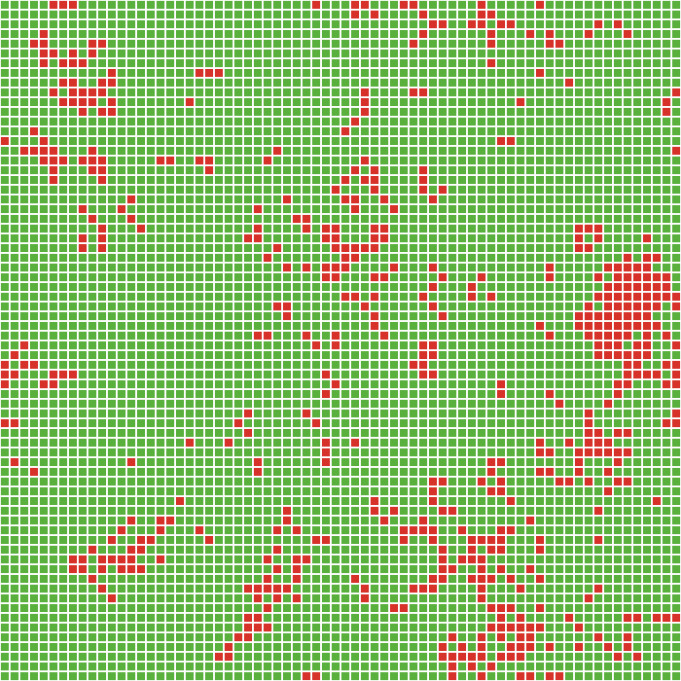
\includegraphics[width=0.5\linewidth]{figures/world.png}}

\renewcommand{\familydefault}{lmss}
%beautiful table
\usepackage[table]{xcolor}
\usepackage{longtable}
\usepackage{tabularx}
%\setlist{nolistsep}
\definecolor{orange}{HTML}{cd8641}
\definecolor{yellow}{HTML}{f0f4b2}
\definecolor{bordeaux}{HTML}{641113}

%%%%%%%%%%%%%%%%%%%%%%%%%%%%%%%%%%%%%%%%%%%%%%%%%%%%%%%%%%%%%%%%%%%%%%%%
%%%%%%%%%%%%%%%%%%%%%%%%%%%%%%%%%%%%%%%%%%%%%%%%%%%%%%%%%%%%%%%%%%%%%%%%
%%%%%%%%%%%%%%%%%%%%%%%%%%%%%%%%%%%%%%%%%%%%%%%%%%%%%%%%%%%%%%%%%%%%%%%%

\begin{document}
\maketitle
\clearpage

\section{Introduction}
The tested hypothesis is the benefit of altruistic strategies for colony growth. The inspiration comes from \citet{bats}, who revealed how \textit{Vampire Bats} demonstrate altruistic behaviour towards other members of the same species who are not strictly related to them. The goal of this research is to prove that some altruistic strategies are selected by specific environments. While it is acknowledged that the simulation environment used in this report is different from the corresponding real world example, the aim of the experiment is to extract variables which affect colony growth in the context of altruism.\\

\citet{dawkins} provides an interesting metaphor for altruistic and selfish behaving entities within a population; the former are called \textit{``suckers"}, the latter \textit{``cheats"}. In the chapter \textit{``You scratch my back, I'll ride on yours"} \cite[p. 165]{dawkins}, he explains how ``cheats" can take advantage of ``suckers" by simply not returning favours. The ultimate consequence of this scenario is the extinction of altruistic behaviour (or its recurring shrinking and expansion).\\

The current project shows how altruistic behaviour, like the one described by \citet{bats}, apply when resources are scarce, while ``cheats", described by \citet{dawkins}, emerge and take over when there are less threats to survival.

%%%%%%%%%%%%%%%%%%%%%%%%%%%%%%%%%%%%%%%%%%%%%%%%%%%%%%%%%%%%%%%%%%%%%%%%
%%%%%%%%%%%%%%%%%%%%%%%%%%%%%%%%%%%%%%%%%%%%%%%%%%%%%%%%%%%%%%%%%%%%%%%%
%%%%%%%%%%%%%%%%%%%%%%%%%%%%%%%%%%%%%%%%%%%%%%%%%%%%%%%%%%%%%%%%%%%%%%%%

\section{Approach}
While \citet{smaldino} demonstrate that, for certain conditions, cooperative behaviour is worse in harsh environments and better in safe ones, the opposite is argued in this report. As stated by \citet[p. 312]{bryson}, simulations are strictly theoretical and can in no case simulate any kind of realistic real-world situation. Therefore, changing a single heuristic  can flip the simulation outcomes, which is what was done in this report.\\

A rational rule-base was constructed with respect to simulation of real-world behaviour. A rule which introduces chance of suicide has been added to \citeauthor{smaldino}'s simulation and will be referred to as \textit{``altruistic suicide''}. This suicidal heuristic is inspired by \citet{bats} and the Vampire Bat's altruistic behaviour. It is intended to be a simplification of altruistic behaviour observed in nature. The assumption behind it is that any altruistic act, puts the entity committing it at risk, as clarified by \citet[p. 451]{smaldino}. This \textit{altruistic suicide} strategy requires part of the population to die and share its resources (its corpse) with the remaining entities in the form of energy.\\

Additional changes made to \citet{smaldino}'s original simulation rules include the removal of the prisoner's dilemma paradigm. The new rules make it so that any interaction between agents generate $+2$ energy units for each communication. The other modification to the code is a pre-defined probability of triggering an \textit{altruistic suicide} at each tick.\\

In the simulation, the population of agents is split between defectors, who do not commit \textit{altruistic suicide}, and cooperators, who do commit \textit{altruistic suicide}. The resources resulting from an \textit{altruistic suicide} are only shared with other cooperative, suicidal entities, not with the selfish part of the population.\\

The experiment consists in testing the speed at which the maximum population is reached, measured in terms of ticks. Throughout the experiment, two variables are tested: the \textit{cost of living} and the \textit{suicide rate}. The initial population consists of 100 agents, with a 50\% split of cooperators and defectors. The world limit is naturally bounded by the 70x70 world size. The tick value is recorded and plotted when the population size reaches $N=4900$.\\

The simulation is conducted in \textit{NetLogo 6.0.3} using a modified version of \cite{smaldino}'s code. Nine runs are carried out using varying \textit{costs of living} and \textit{suicide rates}. The \textit{suicide rate} is used as an indicator of how altruistic the cooperators are (1 being the most and 0 being the least altruistic).

%%%%%%%%%%%%%%%%%%%%%%%%%%%%%%%%%%%%%%%%%%%%%%%%%%%%%%%%%%%%%%%%%%%%%%%%
%%%%%%%%%%%%%%%%%%%%%%%%%%%%%%%%%%%%%%%%%%%%%%%%%%%%%%%%%%%%%%%%%%%%%%%%
%%%%%%%%%%%%%%%%%%%%%%%%%%%%%%%%%%%%%%%%%%%%%%%%%%%%%%%%%%%%%%%%%%%%%%%%

\section{Results}
\label{sec:results}

The results of the nine simulation runs are plotted in a 3D histogram (see Figure \ref{fig:3d-histogram}), where the height of the bars is the number of ticks needed to reach a population of $N=4900$.

\begin{figure}[!htbp]
\centering
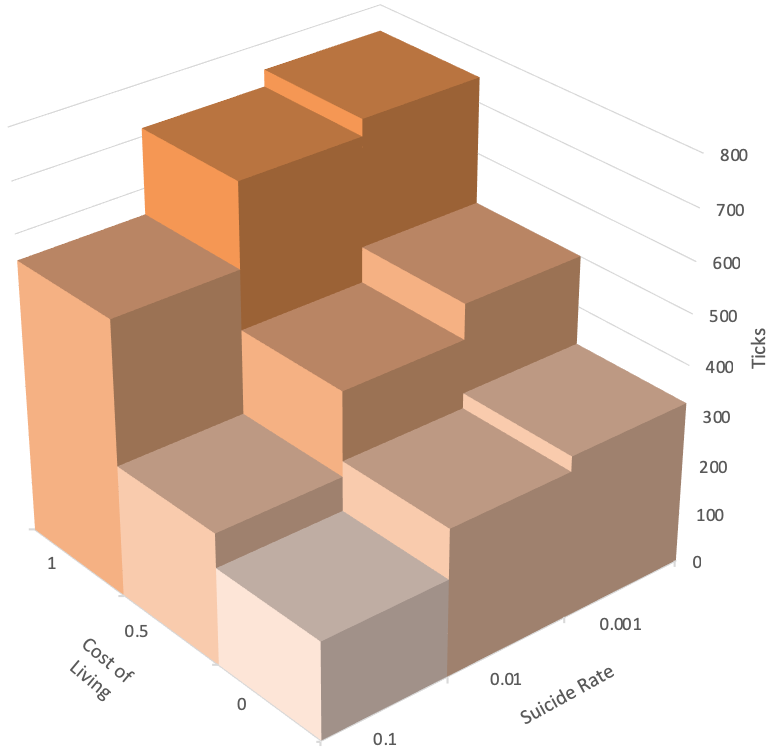
\includegraphics[scale=0.6]{figures/3d_histogram.png}
\caption{Experiment results.}
\label{fig:3d-histogram} 
\end{figure}

The 3D histogram clearly demonstrates that the higher the suicide rate, the quicker the population reaches the maximum threshold, meaning a population that cooperates evolves more quickly than a selfish one. Similarly, the lower the cost of living, the quicker the population evolves, meaning harsh environment conditions hinder a population's growth. The results of the experiment show that altruism (higher suicide rate) helps countering the environment's harsh conditions, allowing the population to grow more quickly. The histogram also betrays a second correlation between the changes in cost of living for lower ranges (from 0 to 0.5), showing a boosting effect for population growth caused by higher suicide rates.

%%%%%%%%%%%%%%%%%%%%%%%%%%%%%%%%%%%%%%%%%%%%%%%%%%%%%%%%%%%%%%%%%%%%%%%%
%%%%%%%%%%%%%%%%%%%%%%%%%%%%%%%%%%%%%%%%%%%%%%%%%%%%%%%%%%%%%%%%%%%%%%%%
%%%%%%%%%%%%%%%%%%%%%%%%%%%%%%%%%%%%%%%%%%%%%%%%%%%%%%%%%%%%%%%%%%%%%%%%

\section{Discussion}

There is a limit to how much \textit{altruistic suicide} contributes to growth. However, this is not reflected by this simulation for high suicide rates due to the intrinsic to the logic of the simulation rules.\\

Focusing on the results from Section \ref{sec:results}, it can be observed that the maximum population is mostly reached thanks to the altruist half. The following factors may play a role in this observation:
\begin{enumerate}
    \item birth energy threshold
    \item net-positive neighbour benefit
    \item \textit{altruistic suicide} energy income
\end{enumerate}
This means that a slight energy-wise advantage favours birth rates from the start. This generates early localised clusters of cooperators which generate more energy than smaller clusters (because of the modified prisoner's dilemma), thus generating more children, more suicides and, consequently, more localisation again. This virtuous cycle maximises growth. Therefore, maximum population is reached fairly quickly thanks to cooperators. Once total world coverage occurs, a stable condition is reached where energy procurement is not a problem, thanks to the updated prisoner's dilemma paradigm. The main take on this is that population growth is maximised in safe environments where populations are more altruistic.\\

Once world coverage is first reached, population growth is no longer required. With cooperators still committing \textit{altruistic suicide}, cells get freed up on the grid and can then be replaced by both defectors or cooperators. As this effect keeps occurring, the altruist population will slowly shrink and eventually be fully replaced by defectors before going extinct, similarly to \citet{dawkins} explanations. But this is just yet another side effect of the experiment which is not considered in the hypothesis.

%%%%%%%%%%%%%%%%%%%%%%%%%%%%%%%%%%%%%%%%%%%%%%%%%%%%%%%%%%%%%%%%%%%%%%%%
%%%%%%%%%%%%%%%%%%%%%%%%%%%%%%%%%%%%%%%%%%%%%%%%%%%%%%%%%%%%%%%%%%%%%%%%
%%%%%%%%%%%%%%%%%%%%%%%%%%%%%%%%%%%%%%%%%%%%%%%%%%%%%%%%%%%%%%%%%%%%%%%%

\section{Conclusion}
The effectiveness of population growth was tested with different rule-bases and different gradations of altruistic behaviour across different environments. The conclusion is that altruistic wealth redistribution among cooperators is beneficial to population growth.

%%%%%%%%%%%%%%%%%%%%%%%%%%%%%%%%%%%%%%%%%%%%%%%%%%%%%%%%%%%%%%%%%%%%%%%%
%%%%%%%%%%%%%%%%%%%%%%%%%%%%%%%%%%%%%%%%%%%%%%%%%%%%%%%%%%%%%%%%%%%%%%%%
%%%%%%%%%%%%%%%%%%%%%%%%%%%%%%%%%%%%%%%%%%%%%%%%%%%%%%%%%%%%%%%%%%%%%%%%

\raggedright
\bibliographystyle{apalike}
\bibliography{bibliography}

\end{document}